\chapter*{2 Versuchsdurchführung und Auswertung}
\addcontentsline{toc}{chapter}{2 Versuchsdurchführung und Auswertung}
\setcounter{chapter}{2}
\setcounter{section}{0}
\setcounter{subsection}{0}

\section{Versuch 1 - Signaldarstellung mit dem Analog-Oszilloskop}

    \subsection{Versuchsaufbau und -durchführung}
    
        Im ersten Versuch sollten wir uns mit den Analog-Oszilloskop vertraut machen.Der Betreuer gibt uns ein Signal vor, welches wir mit dem Analog-Oszilloskop untersuchen sollten. Es sollen die Einstellungen am Oszilloskop, Charakteristika des Signals und eine Skizze des Signal notiert werden. Es soll außerdem der Größtfehler berechnet werden.
        
    \subsection{Ergebnisse}

        Um das Signal gut auf dem Bildschirm erkennen zu können, haben wir uns für folgende Einstellung am Oszilloskop entschieden:
   
        \begin{itemize}
            \item Time/Div: $5\ \mathrm{\mu s}$
            \item Volt/Div: $0.5\ \mathrm{V}$
        \end{itemize}

        Das Schirmbild sieht wie folgt aus:

        \begin{figure}[H]
            \centering
            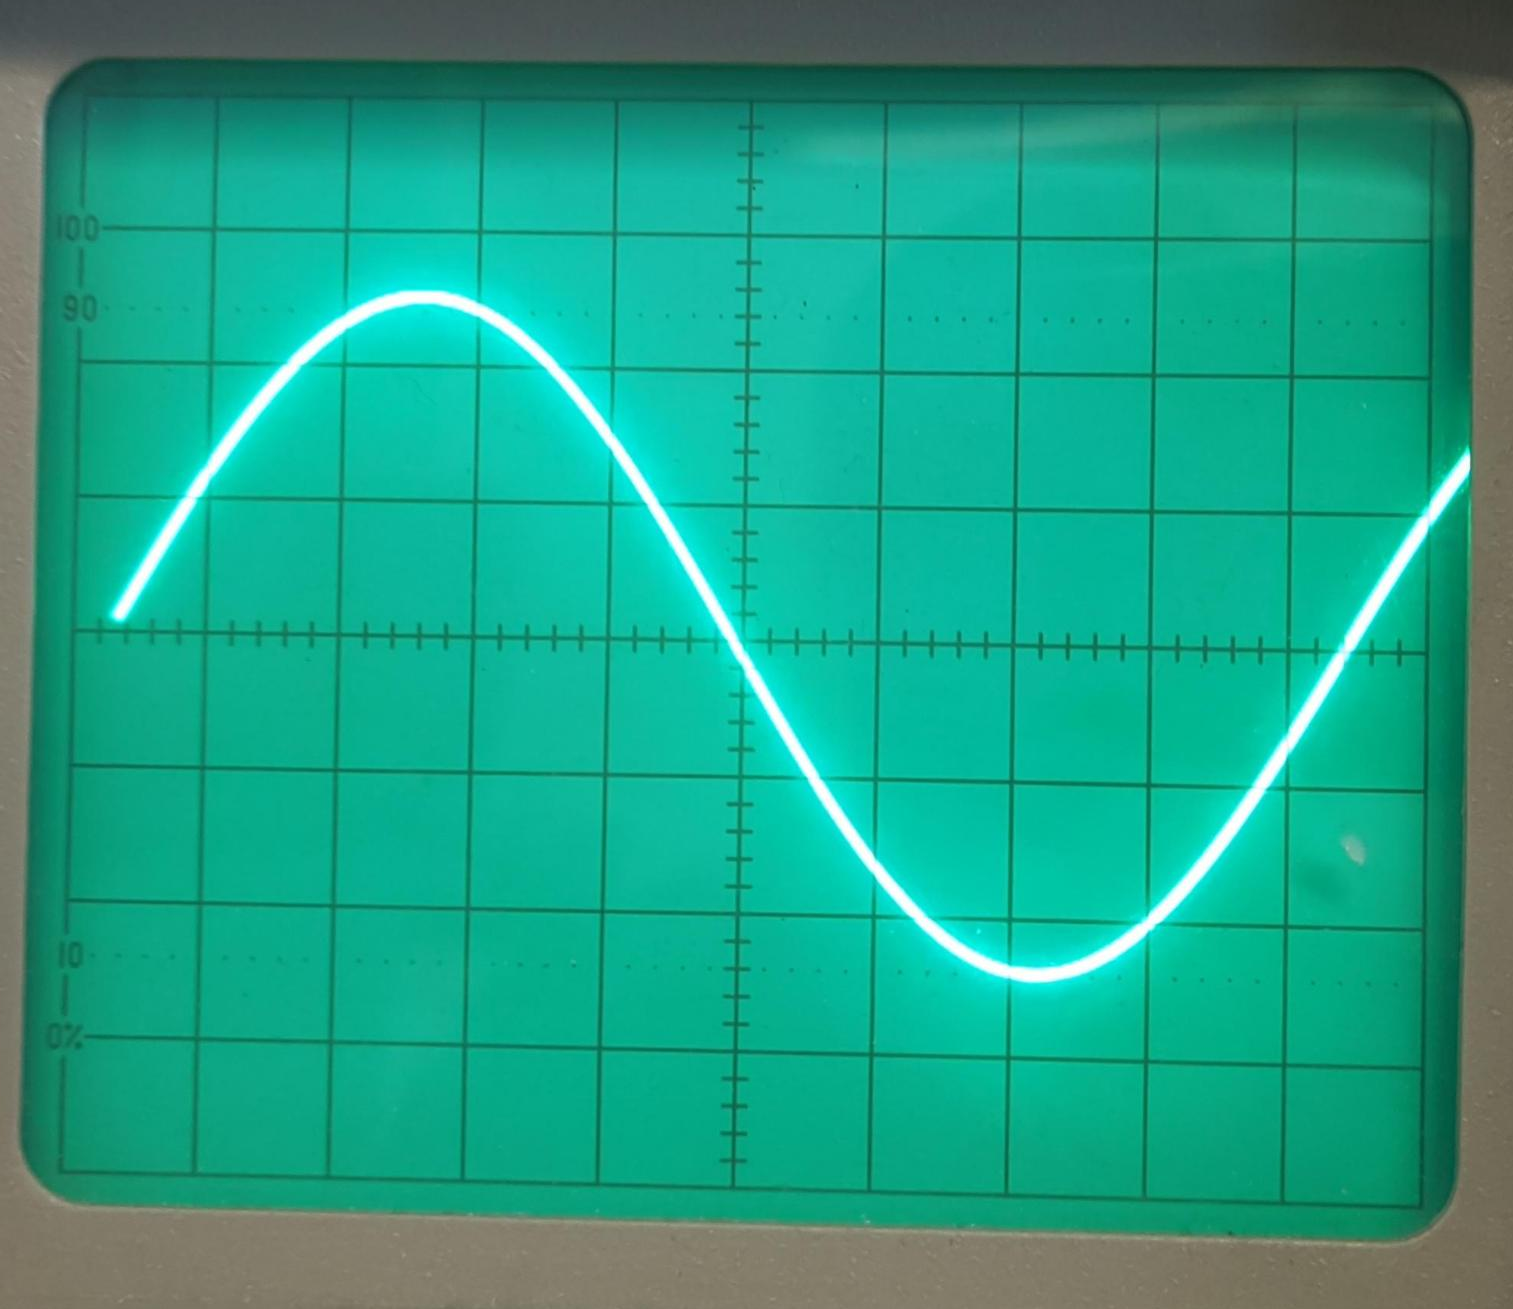
\includegraphics[width=0.6\textwidth]{bilder/Versuch_1.png}
            \caption{Schirmbild des vorgegebenen Signals}
            \label{fig:Versuch1_Schirmbild}
        \end{figure}

        Die folgenden Werte können nun aus der Graphik \ref{fig:Versuch1_Schirmbild} abgelesen werden:

        \begin{table}[H]
            \centering
            \caption{Messwerte des vorgegebenen Signals}
            \vspace*{1em}
            \begin{tabular}{|l|l|}
                \hline
                \textbf{Größe} & \textbf{Wert}\\
                \hline
                \hline
                Amplitude $U_0$ & $1.2 \pm 0.5\ \mathrm{V}$\\
                \hline
                Periodendauer $T$ & $45 \pm 5 \mathrm{\mu s}$\\
                \hline
            \end{tabular}
            
            \label{tab:Versuch1_Messwerte}
        \end{table}
        
        Die Frequenz $f$ des Signals berechnet sich dann wie folgt:

        \begin{equation}
            \begin{aligned}
                f &= \frac{1}{T}\\
                  &= \frac{1}{45\ \mathrm{\mu s}}\\
                  &= 21.7\ \mathrm{kHz}
            \end{aligned}
            \label{eq:Versuch1_Frequenz}
        \end{equation}

        Der Größtfehler der Frequenz berechnet sich wie folgt:

        \begin{equation}
            \begin{aligned}
                \Delta f &= \left|\frac{1}{T^{2}}\right| \cdot \Delta T\\
                         &= \frac{1}{(45\ \mathrm{\mu s})^{2}} \cdot 5\ \mathrm{\mu s}\\
                         &= 0.1\ \mathrm{kHz}
            \label{eq:Versuch1_Frequenz_Fehler}
            \end{aligned}
        \end{equation}
            
        Der Größtfehler der Frequenz beträgt nach \ref{eq:Versuch1_Frequenz_Fehler} $0.1\ \mathrm{kHz}$. Die Frequenz des Signals beträgt also $21.7 \pm 0.1\ \mathrm{kHz}$.
    
    \subsection{Diskussion}

    Die vom Betreuer vorgegebene Frequenz beträgt $20\ \mathrm{kHz}$. Die von uns gemessene Frequenz beträgt $21.7 \pm 0.1\ \mathrm{kHz}$. Die Abweichung beträgt also $1.7\ \mathrm{kHz}$. Dieser Fehler ist unter anderem auf die Ungenauigkeit des Oszilloskops zurückzuführen welche schon länger nichtmehr kalibriert wurden. Eine weitere Fehlerquelle kann die Ungenauigkeit beim Ablesen der Werte sein. Zum Beispiel dann wenn die Sinuswelle zwischen zwei Skalenstrichen durch läuft.
    
\section{Versuch 2 - Impedanzmessung an Widerstand, Kondensator und Spule}
    
    \subsection{Versuchsaufbau und -durchführung}
        
        In Versuch 2 sollen wir die im Stromkreis \ref{fig:Versuch2_Schaltbild} angegebenen Bauteile messen und bestimmen. Aus der Kombination von bekanntem Widerstand $R_{\mathrm{m}}$ und unbekanntem Zweipol $Z$ lässt sich mit verschiedenen Werten der Widerstand und andere Eigenschaften des unbekannten Zweipols bestimmen. Für den unbekannten Zweipol werden die verschiedenen Bauteile, Widerstand, Kondensator und Spule eingegesetzt.

        \begin{figure}[H]
            \centering
            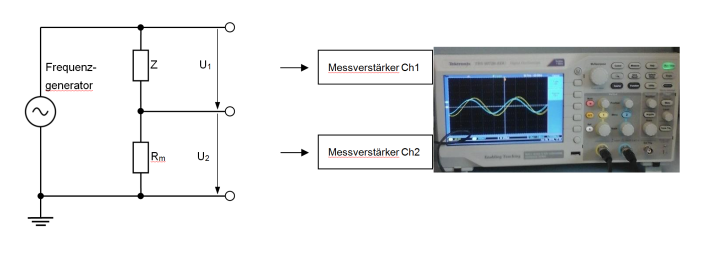
\includegraphics[width=0.8\textwidth]{bilder/Versuch2_Aufbau.png}
            \caption{Schaltbild des Versuchsaufbaus, wir verwenden $U_m$ was hier $U_2$ entspricht \\ und $U_z$ was hier $U_1$ entspricht.}
            \label{fig:Versuch2_Schaltbild}
        \end{figure}

    \subsection{Ergebnisse}

        \subsubsection{Widerstand}
         \label{sec:Versuch2_Widerstand}

            \begin{table}[H]
                \centering
                \caption{Messwerte des Widerstands}
                \vspace{1em}
                \begin{tabular}{|l|l|l|}
                    \hline
                    $U_m$ in $\mathrm{mV}$ & $U_z$ in $\mathrm{mV}$ & $R_{m}$ in $\Omega$\\
                    \hline
                    \hline
                    $460 \pm 40$ & $560 \pm 40$ & $82$\\
                    \hline
                \end{tabular}
                \label{tab:Versuch2_Widerstand}
            \end{table}

            Mit diesen Werten und folgender Formel lässt sich nun der Widerstand $R_{\mathrm{z}} = |Z|$ des unbekannten Zweipols berechnen:

            \begin{equation}
                \frac{U_{\mathrm{m}}}{U_{\mathrm{z}}} = \frac{R_{\mathrm{m}}}{|Z|}
                \label{eq:Versuch2_Widerstand_Formel}
            \end{equation}
            
            \begin{equation}
                \begin{aligned}
                    R_{\mathrm{z}} = |Z| &= \frac{U_{\mathrm{z}}}{U_{\mathrm{m}}} \cdot R_{\mathrm{m}}\\
                                   &= \frac{560\ \mathrm{mV}}{460\ \mathrm{mV}} \cdot 82\ \mathrm{\Omega}\\
                                   &= 99.83\ \mathrm{\Omega}
                \end{aligned}
                \label{eq:Versuch2_Widerstand}
            \end{equation}

            Der Größtfehler beträgt:

            \begin{equation}
                \begin{aligned}
                    \Delta |Z| &= \left|\frac{R_{m} U_{z}}{U_{m}} \right| \cdot \Delta U_{m} + \left|\frac{R_{m}}{U_{m}} \right| \cdot \Delta U_{z}\\
                               &= \left|\frac{82\ \mathrm{\Omega} \cdot 560\ \mathrm{mV}}{460\ \mathrm{mV}} \right| \cdot 40\ \mathrm{mV} + \left|\frac{82\ \mathrm{\Omega}}{460\ \mathrm{mV}} \right| \cdot 40\ \mathrm{mV}\\
                               &= 19.13\ \mathrm{\Omega}
                \end{aligned}
                \label{eq:Versuch2_Widerstand_Fehler}
            \end{equation}

        \subsubsection{Kondensator}
        \label{sec:Versuch2_Kondensator}
            
            Als nächstes wird das unbekannte Bauteil durch einen Kondensator ersetzt. Die Messwerte befinden sich in folgender Tabelle:

            \begin{table}[H]
                \centering
                \caption{Messwerte des Kondensators}
                \vspace{1em}
                \begin{tabular}{|l|l|l|l|}
                    \hline
                    $U_{\mathrm{m}}$ in $\mathrm{V}$ & $U_{\mathrm{z}}$ in $\mathrm{V}$ & $R_{\mathrm{m}}$ in $\mathrm{\Omega}$ & $T_{\mathrm{z}}$ in $\mathrm{\mu s}$\\
                    \hline
                    \hline
                    $0.9\ \mathrm{V}$ & $0.38\ \mathrm{V}$ & $82\ \mathrm{\Omega}$ & $1000\ \mathrm{\mu s}$\\
                    \hline
                \end{tabular}
                \label{tab:Versuch2_Kondensator}
            \end{table}

            Mit diesen Werten lassen sich nun die Kapazität und die Phasenverschiebung bestimmen.
            
            Zunächst bestimmen wir die Frequenz $f$ des Signals:

            \begin{equation}
                \begin{aligned}
                    f &= \frac{1}{T_{\mathrm{z}}}\\
                      &= \frac{1}{1000\ \mathrm{\mu s}}\\
                      &= 1000\ \mathrm{Hz}
                \end{aligned}
                \label{eq:Versuch2_Kondensator_Frequenz}
            \end{equation}

            Danach berechnen wir die Winkelgeschwindigkeit $\omega$:

            \begin{equation}
                \begin{aligned}
                    \omega &= 2 \pi f\\
                           &= 2 \pi \cdot 1000\ \mathrm{Hz}\\
                           &= 6283.19\ \mathrm{Hz}
                \end{aligned}
                \label{eq:Versuch2_Kondensator_Winkelgeschwindigkeit}
            \end{equation}

            Damit können wir abschließend die Kapzität $C$ des Kondensators berechnen:

            \begin{equation}
                \begin{aligned}
                    C &= \frac{1}{\omega \cdot |Z|}\\
                      &= \frac{1}{6283.19\ \mathrm{Hz} \cdot 82\ \mathrm{\Omega}}\\
                      &= 4.6 \cdot 10^{-6}\ \mathrm{F}
                \end{aligned}
                \label{eq:Versuch2_Kondensator_Kapazität}
            \end{equation}

            Anschließend können wir die Phasenverschiebung $\varphi$ berechnen:

            \begin{equation}
                \begin{aligned}
                    \varphi &= \frac{t}{T} \cdot 360^{\circ}\\
                         &= \frac{-250\ \mathrm{\mu s}}{1000\ \mathrm{\mu s}} \cdot 360^{\circ}\\
                         &= -90^{\circ}
                \end{aligned}
                \label{eq:Versuch2_Kondensator_Phasenverschiebung}
            \end{equation}

            Zum Schluss berechnen wir noch den Größtfehler der Phasenverschiebung:

            \begin{equation}
                \begin{aligned}
                    \Delta \varphi &= \left|\frac{360^{\circ}}{T_{\mathrm{z}}}\right| \cdot \Delta t + \left|\frac{360^{\circ} \cdot t}{T_{\mathrm{z}}^{2}}\right| \cdot \Delta T\\
                                   &= \left|\frac{360^{\circ}}{1000\ \mathrm{\mu s}}\right| \cdot 50\ \mathrm{\mu s} + \left|\frac{360^{\circ} \cdot (-250\ \mathrm{\mu s})}{(1000\ \mathrm{\mu s})^{2}}\right| \cdot 50\ \mathrm{\mu s}\\
                                   &= 13.5^{\circ}
                \end{aligned}
                \label{eq:Versuch2_Kondensator_Phasenverschiebung_Fehler}
            \end{equation}

        \subsubsection{Spule}
        \label{sec:Versuch2_Spule}
            
            Um die Phasenverschiebung $\varphi$ der Spule zu bestimmen, müssen wir die Periodendauer $T_{\mathrm{z}}$ und die Phasenverschiebung $t$ messen.
            Die Periodendauer $T_{\mathrm{z}}$ beträgt $100\ \mathrm{\mu s}$, die Phasenverschiebung $t$ beträgt $25\ \mathrm{\mu s}$. Der Fehler für $T_{\mathrm{z}}$ und $t$ beträgt $5\ \mathrm{\mu s}$.

            Die Phasenverschiebung $\varphi$ berechnet sich dann wie folgt:

            \begin{equation}
                \begin{aligned}
                    \varphi &= \frac{t}{T} \cdot 360^{\circ}\\
                         &= \frac{25\ \mathrm{\mu s}}{100\ \mathrm{\mu s}} \cdot 360^{\circ}\\
                         &= 90^{\circ}
                \end{aligned}
                \label{eq:Versuch2_Spule_Phasenverschiebung}
            \end{equation}

            Der Größtfehler wird mit der gleichen Formel wie bei dem Kondensator berechnet:

            \begin{equation}
                \begin{aligned}
                    \Delta \varphi &= \left|\frac{360^{\circ}}{T_{\mathrm{z}}}\right| \cdot \Delta t + \left|\frac{360^{\circ} \cdot t}{T_{\mathrm{z}}^{2}}\right| \cdot \Delta T\\
                                   &= \left|\frac{360^{\circ}}{100\ \mathrm{\mu s}}\right| \cdot 5\ \mathrm{\mu s} + \left|\frac{360^{\circ} \cdot 25\ \mathrm{\mu s}}{(100\ \mathrm{\mu s})^{2}}\right| \cdot 5\ \mathrm{\mu s}\\
                                   &= 22.5^{\circ}
                \end{aligned}
                \label{eq:Versuch2_Spule_Phasenverschiebung_Fehler}
            \end{equation}
             \subsection{Diskussion}
             \textcolor{red}{TODO Verstehe das mit dem Runden nicht.}
             Zu \ref{sec:Versuch2_Widerstand} lässt sich sagen das unser berechneter Widerstand von $99.83 \pm 19.13\ \mathrm{\Omega}$ sehr nah an dem tatsächlichen Widerstand von $110\ \mathrm{\Omega}$ liegt. Die Maximale Abweichung beträgt hier also $29.30\ \mathrm{\Omega}$.

             \noindent Zu \ref{sec:Versuch2_Kondensator} lässt sich sagen das die Phasenverschiebung von $-90^{\circ} \pm 13.5^{\circ}$ sehr nah an der tatsächlichen Phasenverschiebung von $-90^{\circ}$ liegt. Der Fehler entspricht also dem Größtfehler von $13.5^{\circ}$.

             \noindent Zu \ref{sec:Versuch2_Spule} lässt sich sagen das die gemessene Phasenverschiebung von $-90^{\circ} \pm 22.5^{\circ}$ sehr nah an der tatsächlichen Phasenverschiebung von $90^{\circ}$ liegt. Der Fehler entspricht also dem Größtfehler von $22.5^{\circ}$. 

             \noindent Die Abweichungen der Fehler kamen vorallem durch Ungenauigkeiten beim ablesen vom Oszilloskop zustande. Die Linie ist hier nunmal keine gerade Sinuswelle sondern eine \"zitternde\" Kurve welche das ablesen erschwert. 

\section{Versuch 3 - Impedanzmessung an einem unbekannten Zweipol}
    
    \subsection{Versuchsaufbau- und durchführung}

        Im letzten Versuch sollen wir die Charakteristika von zwei unbekannten Zweipolen bestimmen. Dazu wird eine Tabelle mit verschiedenen Frequenzen vorgegeben. Anhand der Messwerte soll bestimmt werden, welche zwei Zweipole und in welcher Art und Weise sie verschaltet sind.

    \subsection{Ergebnisse}
    
        Die gemessenen Werte befinden sich in folgender Tabelle:

        \begin{table}[H]
            \centering
            \caption{Messwerte Versuch 3}
            \vspace{0.5em}
            \begin{tabular}{|l||l|l|l|l|l|l|l|l|}
                \hline
                $f$[Hz] & $U_m$[mV]  & $U_z$[mV] & $R_{m}$[$\Omega$] & $|Z|$[$\Omega$] & $t$ [$\mu$s] & $T$[ms] & $\omega$[Hz] & $\phi$[°] \\
                \hline
                \hline
                200,00   & 22,50  & 1000,00 & 82,00 & 3644,44 & -500,00 & 5000,00 & 1256,64   & -36,00 \\
                \hline
                400,00   & 20,00  & 1000,00 & 82,00 & 4100,00 & -200,00 & 2500,00 & 2513,27   & -28,80 \\
                \hline
                1000,00  & 20,00  & 1000,00 & 82,00 & 4100,00 & -100,00 & 1000,00 & 6283,19   & -36,00 \\
                \hline
                2000,00  & 28,00  & 1000,00 & 82,00 & 2928,57 & -75,00  & 500,00  & 12566,37  & -54,00 \\
                \hline
                4000,00  & 44,00  & 1000,00 & 82,00 & 1863,64 & -50,00  & 250,00  & 25132,74  & -72,00 \\
                \hline
                10000,00 & 110,00 & 1000,00 & 82,00 & 745,45  & -22,00  & 100,00  & 62831,85  & -79,20 \\
                \hline
                20000,00 & 200,00 & 1000,00 & 82,00 & 410,00  & -11,00  & 50,00   & 125663,71 & -79,20 \\
                \hline
                40000,00 & 400,00 & 1000,00 & 82,00 & 205,00  & -6,00   & 25,00   & 251327,41 & -86,40 \\
                \hline
                80000,00 & 660,00 & 1000,00 & 82,00 & 124,24  & -3,00   & 12,50   & 502654,82 & -86,40\\
                \hline
            \end{tabular}
            \label{tab:Versuch3_Messwerte}
        \end{table}

        \noindent Es lässt sich erkennen, dass ein Widerstand und ein Kondensator parallel geschaltet sind. Warum dies so ist, wird in der Diskussion erläutert.

        \noindent Nun können wir mit folgender Formel die Kapazität des verbauten Kondensators berechnen:
        \textcolor{red}{TODO das gleiche für R}
        \begin{equation}
            \begin{aligned}
                C &= \frac{1}{\omega \cdot |Z|}\\
                  &= \frac{1}{251327\ \mathrm{Hz} \cdot 205\ \mathrm{\Omega}}\\
                  &= 19.4\ \mathrm{nF}
                \label{eq:Versuch3_Kapazität}
            \end{aligned}
        \end{equation}

        Für |Z| wählen wir das |Z|, bei dem $\phi$ am nächsten an -90° ist.

        \begin{figure}[H]
            \begin{subfigure}{0.5\textwidth}
                \centering
                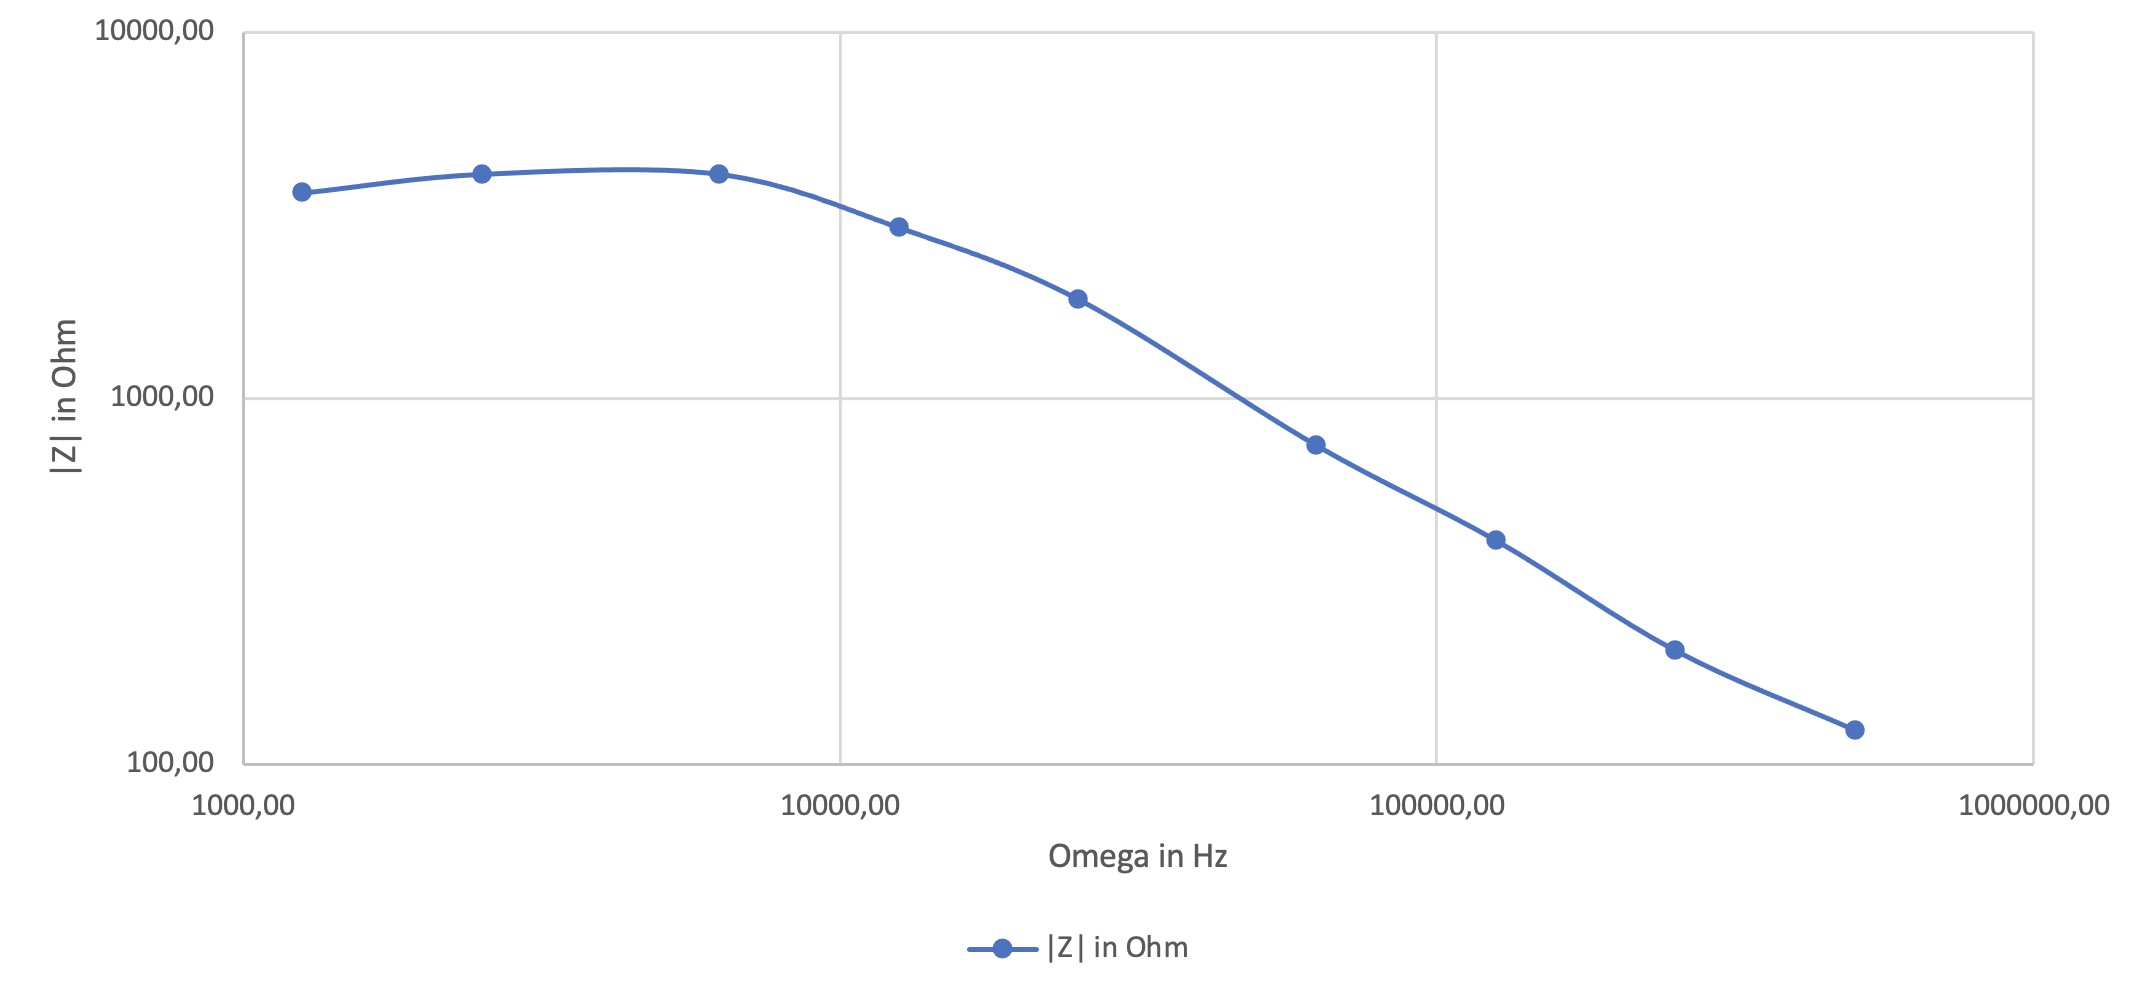
\includegraphics[width=0.9\textwidth]{bilder/Versuch3_1.png}
                \caption{$|Z|$ über $\omega$}
                \label{fig:Versuch3_Messwerte_1}
            \end{subfigure}
            \begin{subfigure}{0.5\textwidth}
                \centering
                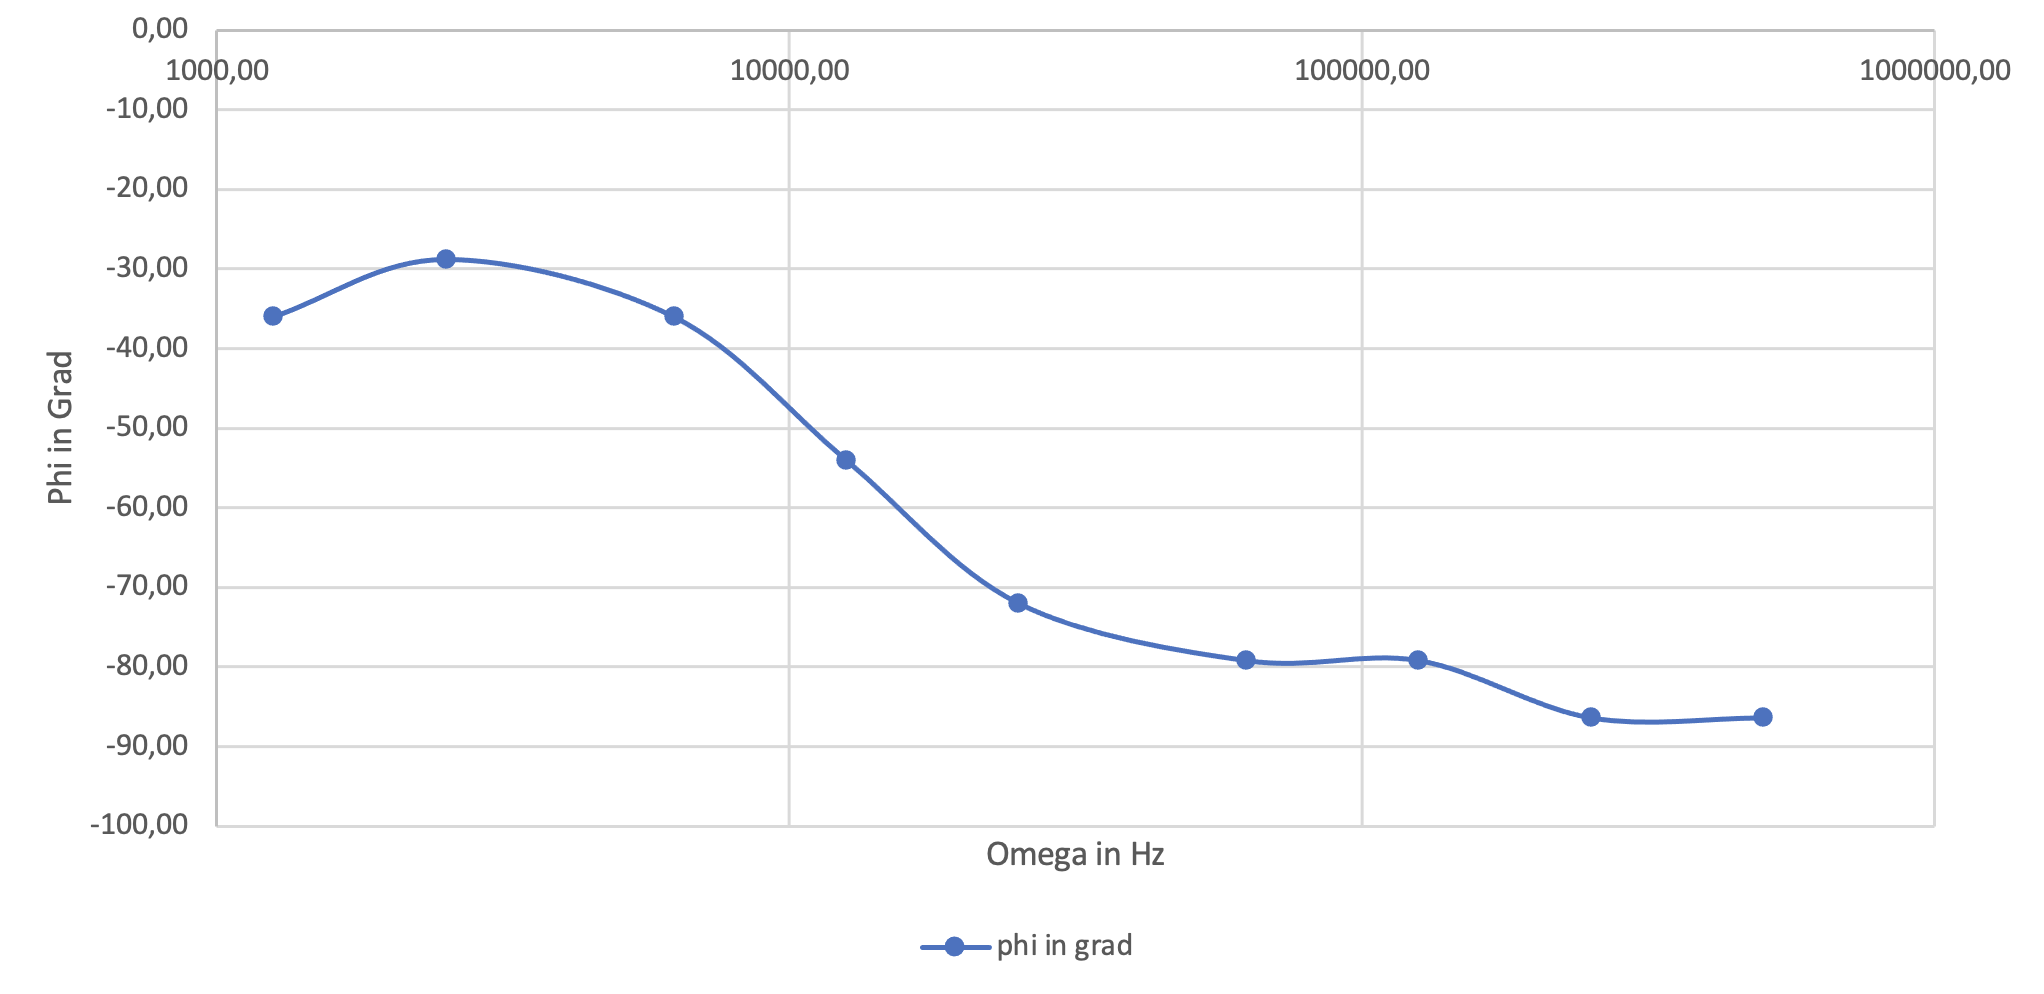
\includegraphics[width=0.9\textwidth]{bilder/Versuch3_2.png}
                \caption{$\varphi$ über $\omega$}
                \label{fig:Versuch3_Messwerte_2}
            \end{subfigure}
        \end{figure}

    \subsection{Diskussion}
    \begin{figure}[H]
        \centering
                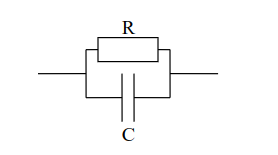
\includegraphics[width=0.3\textwidth]{bilder/2pol.png}
                \caption{2-Pol aus Versuch 3}
                \label{fig:2pol}
    \end{figure}
    Der unbekannten Zweipol den wir bekommen hatten, ist in \ref{fig:2pol} zu sehen. Es handelt sich hierbei um einen Widerstand und einen Kondensator welche parallel geschaltet wurden. Die lässt sich an der Phasenverschiebung erkennen. Aus Versuch \ref{sec:Versuch2_Kondensator} wissen wir das ein Kondensator mit einer Phasenverschiebung von $-90^{\circ}$ zu erkennen ist. Dies zeigt sich in Tabelle \ref{tab:Versuch3_Messwerte} bei 80kHz. Die Phasenverschiebung beträgt hier $-86.4^{\circ}$. Dieser Wert ist sehr nah an $-90^{\circ}$ und lässt sich durch Messungenauigkeiten erklären. Der Widerstand hingegen hat keine Phasenverschiebung und würde sich deshalb ebenfalls in Tabelle \ref{tab:Versuch3_Messwerte} zeigen. Und zwar tritt dies bei 200 Hz auf. Leider kam es hier zu einer großen Ungenauigkeit von $-28.8^{\circ}$ was aber am nächsten an 0 liegt und deshalb als 0 berachtet wurde.\\

    \noindent Die Ungenauigkeit lässt sich durch alte Technik und Ungenaugigkeiten beim ablesen erklären. 
    \textcolor{red}{TODO besser erklären warum parallel und nicht Reihenschaltung}